\section{Results}
\label{sec:results}

The information gathered in the user tests through the questionnaire and the interviews is presented in this section. The full questionnaire and a link to the raw data can be found in Annex \ref{REF HERE} The questionnaire answers are divided in two graphs: Figure \ref{fig:abGraph} summarizes the results of the A/B test-type questions, while Figure \ref{fig:descriptionGraph} contains the results of the questions where the testers where asked to select descriptions from a list to describe each hand version (they were also given the option to write their own description).

\todo[inline]{Reference to questionnaire + interview + raw data link Annex}

Figure \ref{fig:interviewResults} presents the the result of performing a qualitative data analysis of the interview notes. The notes were coded and categorized following an inductive process, meaning that they were created based on the themes of the interview notes \parencite{Burnard2008}, and the number of occurrences of the labels in the notes was counted as a measure of the relevance of each label.

We conducted the test procedure with 10 graduate-level university students (7 men and 3 women). It should be noted that all of the test subjects part of the games program at IT University of Copenhagen, so these results might not be fully representative of the general VR game player/user population.

\begin{figure}[h]
\centering
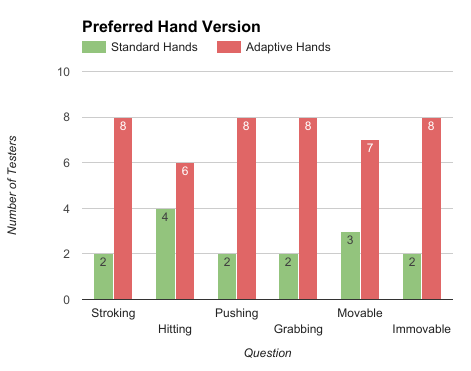
\includegraphics[width=0.8\textwidth]{abGraph.png}
\caption{Graph showing the number of testers that preferred each version of the hands in each of the aspects described by the A/B test-type questions: "With which version did you prefer petting/stroking the creatures?" (Stroking), "With which version did you prefer hitting things?" (Hitting), "With which version did you prefer pushing things?" (Pushing), "With which version did you prefer grabbing things?", (Grabbing), "Which version did you prefer in terms of how they interacted with objects that you could move?" (Movable), "Which version did you prefer in terms of how they interacted with objects that you could NOT move?" (Immovable).}
\label{fig:abGraph}
\end{figure}

The labels in Figure \ref{fig:interviewResults} have the following meanings. In the \textit{Fingers} category, \textit{Stroking Good} means that the tester expressed that the finger adjustment improved the stroking experience: \textit{Hover Good} means that they liked the finger adjustment or hover around movable objects in a general sense. \textit{Impossible Grip} means that they expressed a dislike for the cases when the hands grabbed objects in a way that would be impossible in real life because it would not be possible to get a grip e.g. on a completely flat surface. \textit{Loose Grip} is similar to the previous one, and refers to disliking the cases when they grabbed an object and the hand pose didn't make contact with the object. \textit{Hidden Grab} refers to users expressing a dislike for the Standard hands disappearing when an object is grabbed. \textit{Flat Slap} refers to user's pointing out that because of the finger adjustment or hover around movable objects, hitting the objects with a flat hand wasn't possible. \textit{Unnoticed} refers to the cases when the users didn't notice the finger adjustment in the Adaptive hand. \textit{Inconsistent} means that the tester mentioned the fact that the fingers didn't adjust around immovable objects and were inconsistent in that sense.


In the \textit{Rumble} category, the label \textit{Unpleasant} means that testers expressed that the haptic feedback or rumble given by the controllers was unpleasant to them. \textit{Satisfying} means that the users mentioned that the rumble was satisfying at least in some of the cases when they felt it. \textit{Informative} means that the testers found the rumble informed them of about the virtual environment, virtual events or the environment constraints or "rules". \textit{Innacurate} means that the testers described the rumble as "innacurate", "imprecise" or "unpolished". \textit{Intimate} means that the user considered that the rumble made the touch interaction feel more intimate. \textit{Confusing} means that the user expressed feeling confused about the why the rumble was being produced.

\begin{figure}[H]
\centering
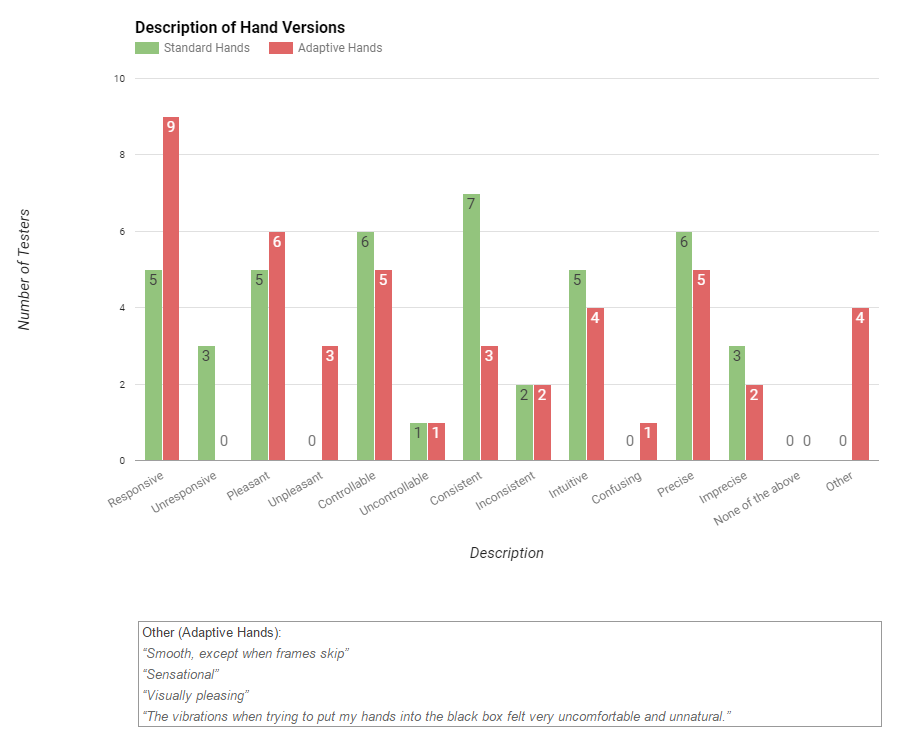
\includegraphics[width=\textwidth]{descriptionGraph2.png}
\caption{Graph of the number of testers that chose each of the words in a list to describe the two versions of the hand that were shown. A few of the testers added descriptions of their own, which are quoted under the graph.}
\label{fig:descriptionGraph}
\end{figure}

In the \textit{Physics} category, \textit{Natural Grab} means that users liked and found it easier with the Adaptive hands to lift objects and manipulate purely using the physics system (e.g. lifting an object by placing their hands on opposite side of the object and moving their hands towards each other) instead of making use of the "artificial" trigger grab mechanic. \textit{Penetration} means that the testers expressed liking the fact that their hands could not move into immovable objects. \textit{Weight} means that the users mentioned that objects seemed to have weight when interacting with them with the Adaptive hands. \textit{Hard Lifting} refers to users expressing that the Natural Grab was better, but not easy enough with the Adaptive hands. \textit{Unnecessary} means that the user expressed not feeling inclined to break the physics rules of the environment, because there were contextual signifiers \parencite{Norman2010} that made each virtual object's affordances clear.

In the \textit{Communication} category, \textit{Wireframe Late} means that the users found that the wireframe version of the Adaptive hand shown when the hand was separated from the controller appeared too late (for example because the controller is inside of a virtual object). \textit{Wireframe Good} means that they found that the wireframe visualization clarified that the system was working as intended and that there was no "bug" when the virtual hands separated from the controller. \textit{No Grab Feedback} means that a user expressed missing some kind of feedback when in the moment when the grab action is completed and the grabbed object is attached to the grabbing hand. \textit{Sound Feedback} means that the user expressed liking the sound effects produced by certain interactions. \textit{Feedback Good} refers to a general positive appreciation of the feedback with the Adaptive hands.

\begin{figure}[H]
\centering
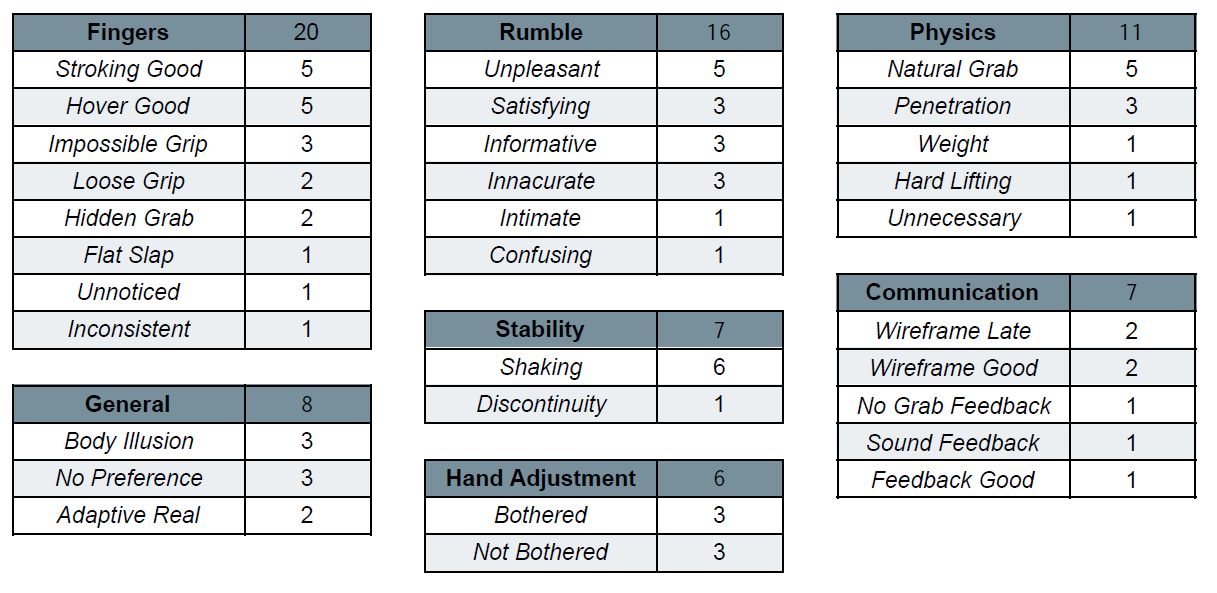
\includegraphics[width=\textwidth]{interviewResults.png}
\caption{Each table shows a category and its labels with the number of mentions found in the interview notes.}
\label{fig:interviewResults}
\end{figure}

Under \textit{Stability}, \textit{Shaking} means that the users noticed and expressed dislike for the cases when the Adaptive hand shook or moved in a "jumpy" fashion when interacting with objects. \textit{Discontinuity} refers to users noticing small discontinuities in the finger movement in some situations.

In the \textit{Hand Adjustment} category, \textit{Bothered} means that the users expressly disliked when the Adaptive hands separated from the controllers in terms of position or rotation (not including finger adjustments). \textit{Not Bothered} means that the users expressly manifested not being bothered or in some cases not noticing when the hands separated from the controller in the previous sense.

Finally, under \textit{General}, \textit{Body Illusion} refers to users expressing that the sometimes found themselves behaving as if they had parts their body that the virtual body didn't have. \textit{No Preference} means that the users expressly recognized that there was "nothing wrong" with the Standard hand or that they had no strong feelings of preference towards either version. \textit{Adaptive Real} refers to users that mentioned that the Adaptive hands felt "more real" to them.

\subsection{Discussion}
\label{subsec:discussion}

Analyze with theory?